\chapter{Lists}\label{CHAP_Lists}

\section{Difficulty: EASY}

\subsubsection*{Exercise 7.E01}
Initialize lists with your five favourite animals/cars/sports/books/foods/whatever else you
want. Display the content of the lists using the {\code{print()}} function.\\


\textit{Hints:
When initializing a non-empty list, list objects are placed inside the square brackets and
separated by commas.}\\[1cm]


% ------------------------------------------------------------------------------


\subsubsection*{Exercise 7.E02}
Copy the following lists into your Jupyter Notebook:
\begin{figure}[H]
		\centering
		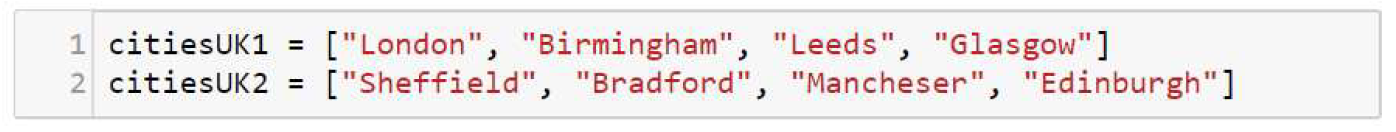
\includegraphics[width=\textwidth]{../IMG/7E02.png} 
\end{figure}
Generate a new list, {\code{citiesUK}}, containing the sum of {\code{citiesUK1}} and {\code{citiesUK2}} then (using list indices where appropriate)
\begin{enumerate}[label=(\alph*)]
	\item Print the entire list to your screen
	\item Print only the third object in the list to your screen
	\item Print the last object in the list to your screen
	\item Change the first object in the list from London to Cardiff then print your list again
	\item Generate a new list containing the cities Birmingham to Manchester using a list slicing operation. Display your new list using the {\code{print()}} function
\end{enumerate}


\textit{Hints:
You can use the {\code{+}} operator to add lists together. Every object in the list is assigned an index. You can access individual objects by calling their index in square brackets behind the list name: {\code{myList[index]}}. You can also generate sub-lists by declaring an index range in square brackets behind the list name: {\code{myList[index1:index2]}}.}\\[1cm]


% ------------------------------------------------------------------------------


\subsubsection*{Exercise 7.E03}
Repeat Exercise 7.E01 but this time start by generating an empty list. Then, using the
{\code{append()}} function, add your 5 favourite animals/cars/sports/books/foods/whatever else
you want to the list. When you’re done display the content of the list.\\


\textit{Hints:
The {\code{append()}} function will add new objects to the end of your list. Remember the full stop when applying a list operator to a list: {\code{listName.FunctionName(arguments)}}.}\\[1cm]


% ------------------------------------------------------------------------------


\subsubsection*{Exercise 7.E04}
Copy the following list into your Jupyter Notebook:
\begin{figure}[H]
		\centering
		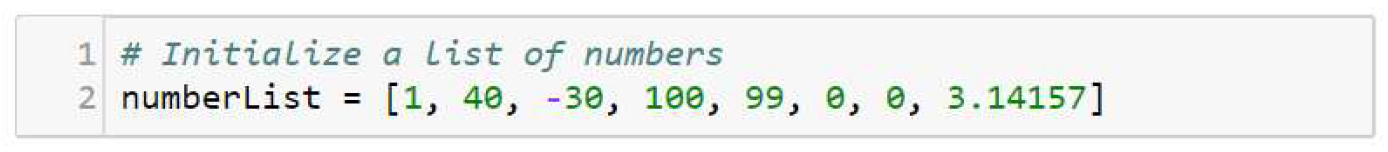
\includegraphics[width=\textwidth]{../IMG/7E04_1.png} 
\end{figure}
Using the {\code{insert(index, object)}} function, keep adding objects to the list until the list content looks like this:
\begin{figure}[H]
		\centering
		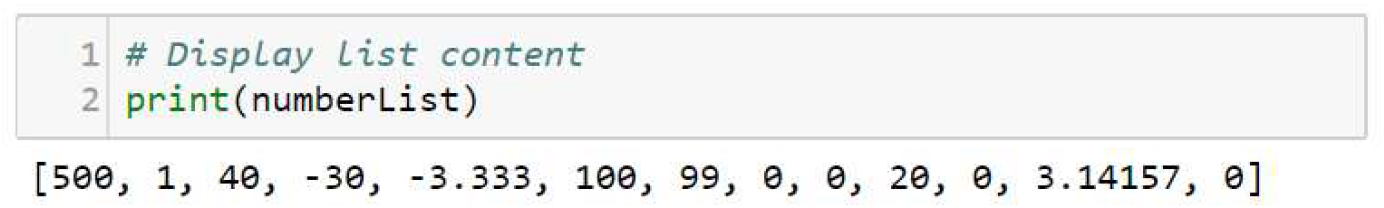
\includegraphics[width=\textwidth]{../IMG/7E04_2.png} 
\end{figure}

\textit{Hints:
Remember that the index assigned to an object in a list might change if you insert a new
object.}\\[1cm]


% ------------------------------------------------------------------------------

\newpage
\subsubsection*{Exercise 7.E05}
Copy the following lists into your Jupyter Notebook
\begin{figure}[H]
		\centering
		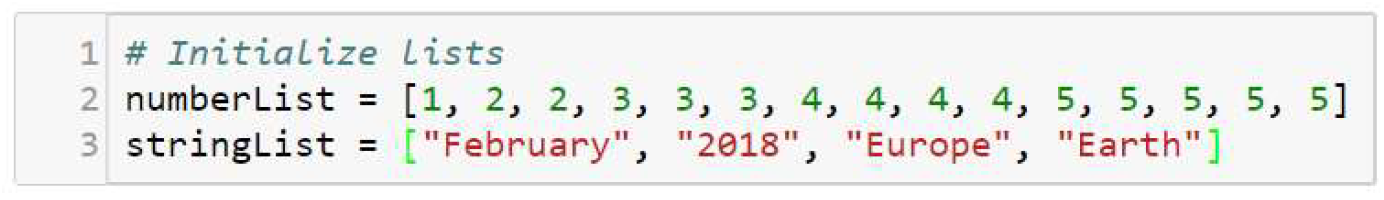
\includegraphics[width=\textwidth]{../IMG/7E05.png} 
\end{figure}
and
\begin{enumerate}[label=(\alph*)]
	\item Use the {\code{remove()}} function to remove the object February from {\code{stringList}}\\
	\item Use the {\code{del}} function to remove the object Earth from {\code{stringList}}\\
	\item Use the {\code{del}} function to remove all number 3s from {\code{numberList}}\\
	\item Use the {\code{remove()}} function to remove all number 4s from {\code{numberList}}\\
\end{enumerate}

\textit{
Hints:
The {\code{del}} function will remove an object by index, the {\code{remove()}} function by content!}\\[1cm]


% ------------------------------------------------------------------------------


\subsubsection*{Exercise 7.E06}
Copy the following list into your Jupyter Notebook:
\begin{figure}[H]
		\centering
		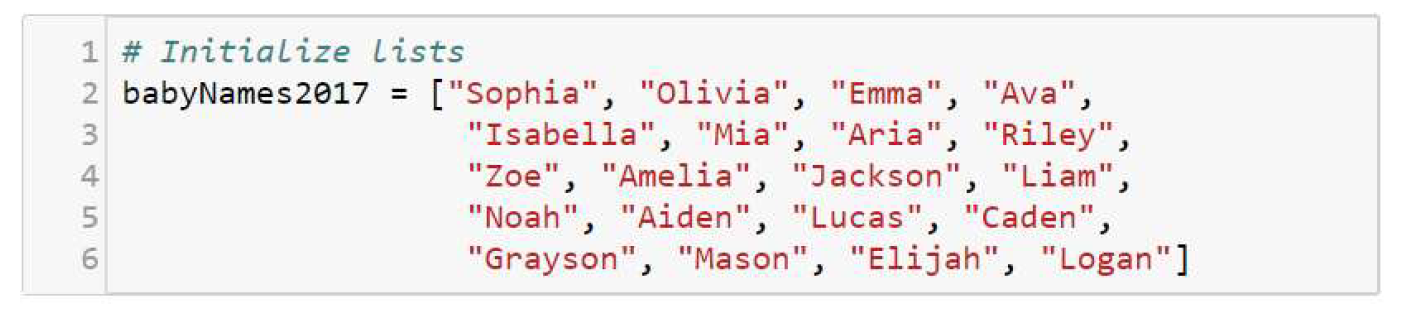
\includegraphics[width=\textwidth]{../IMG/7E06.png} 
\end{figure}
Ask the user for a name and then check whether the name is among the top 20 baby names
of 2017 using the in function.\\


\textit{Hints:
You can simply print the result of the {\code{in}} function to your screen or you can try including an {\code{IF and ELSE}} Statement that prints a message like {\code{"[NAME] was/was not among the top 20 baby names of 2017"}} where [NAME] is a place holder for the user input.
}


% ------------------------------------------------------------------------------





\newpage
\section{Difficulty: MEDIUM}


\subsubsection*{Exercise 7.M01}
List repetition allows you to generate larger lists more easily if objects are repeated within
the list:
\begin{figure}[H]
		\centering
		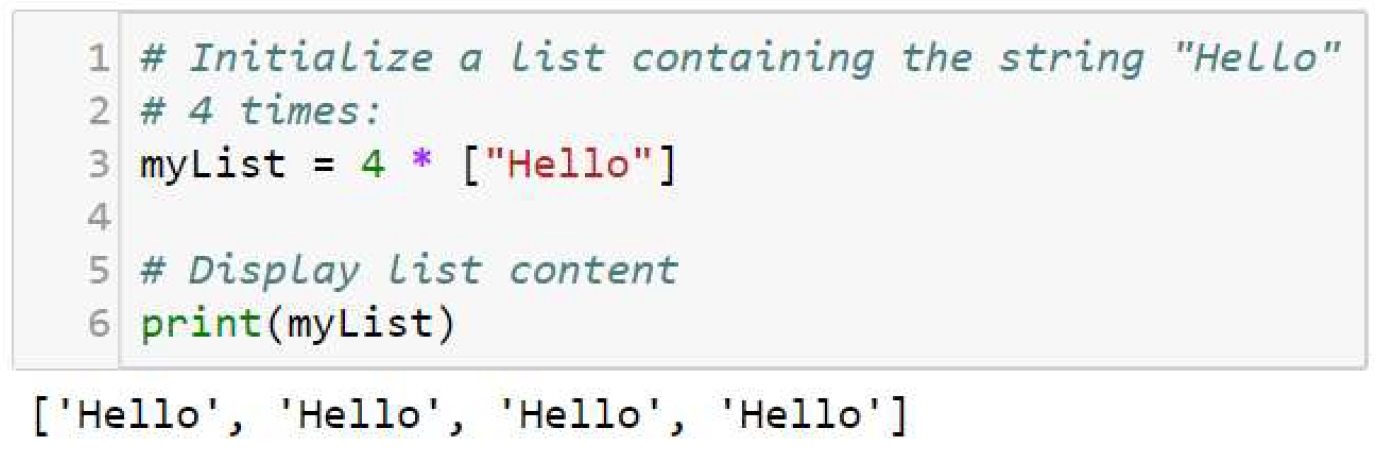
\includegraphics[width=\textwidth]{../IMG/7M01.png} 
\end{figure}

Using repetition, generate a list that contains the number 1 once, the number 2 twice, the
number 3 thrice, the number 4 four times, the number 5 five time, the number 6 six times,
the number 7 seven times, the number 8 eight times, the number 9 nine time, and finally the
number 10 ten times.\\


\textit{Hints:
Remember, you can add lists together using the {\code{+}} operator.}\\[1cm]


% ------------------------------------------------------------------------------


\subsubsection*{Exercise 7.M02}
Copy the following list initializations into your Jupyter Notebook:
\begin{figure}[H]
		\centering
		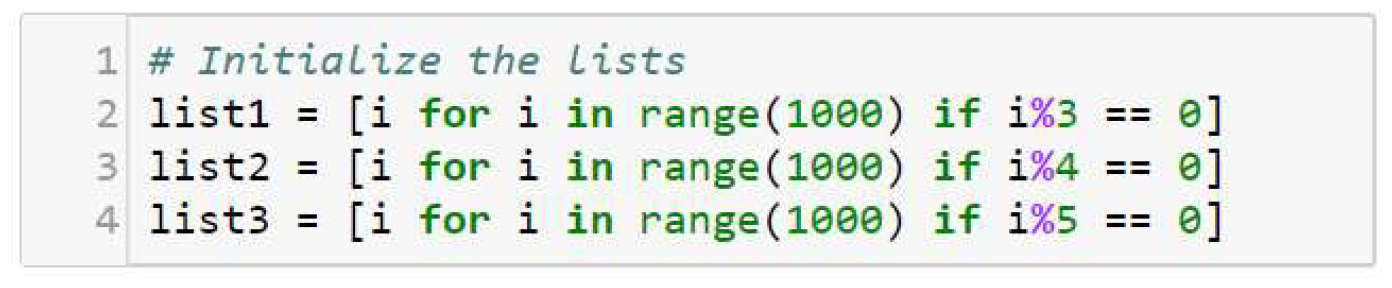
\includegraphics[width=\textwidth]{../IMG/7M02.png} 
\end{figure}
Don’t worry about understanding these lines. What you see above is called list
comprehension which is not part of the syllabus but used here to quickly generate larger
lists for you to work with. The commands will produce:
\begin{itemize}
	\item list1 which stores all the numbers between 0 and 10,000 that are divisible by 3
	\item list2 which stores all the numbers between 0 and 10,000 that are divisible by 4
	\item list3 which stores all the numbers between 0 and 10,000 that are divisible by 5
\end{itemize}

Using the {\code{len()}} function, determine how many objects are contained in each of these lists.\\


\textit{Hints:
Remember, the {\code{len()}} function is not a list operator but a function that works on multiple data types. It’s therefore not initialized the way normal list operators are initialized.}\\[1cm]


% ------------------------------------------------------------------------------


\subsubsection*{Exercise 7.M03}
Initialize the following list you Jupyter Notebook:
\begin{figure}[H]
		\centering
		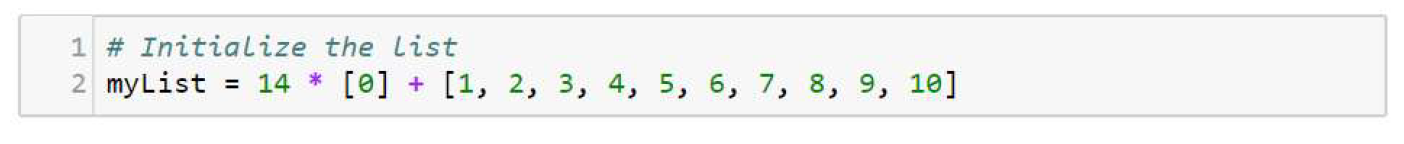
\includegraphics[width=\textwidth]{../IMG/7M03.png} 
\end{figure}
The list you’ve just generated has quite a few 0 objects at the beginning. Instead of removing
all the zeros, use the {\code{index(0)}} function generate a new list containing the none-zero
elements starting with 1.\\


\textit{Hints:
Use the {\code{index()}} function to find the index corresponding to 1, then generate a sub-list from that index to the end of the original list. You might find the {\code{len()}} function useful too.}\\[1cm]


% ------------------------------------------------------------------------------


\subsubsection*{Exercise 7.M04}
In this exercise you will be putting together a shopping list. The initial list should contain the following items:\\
\begin{center}
milk, eggs, red peppers, chicken, apples, onions, bread, coffee, and a cucumber
\end{center}
Using the list operators you have learned so far, perform the following actions on your list:
\begin{enumerate}[label=(\alph*)]
	\item Determine how many items are on your shopping list
	\item Print your shopping list in the following format:\\
{\code{Shopping list:}}\\
\hspace*{5mm}{\code{- [ITEM]}}\\
\hspace*{5mm}{\code{- [ITEM]}}\\
\hspace*{5mm}{\code{…}}\\
where [ITEM] is a place holder for your list objects.
	\item Add butter and spring onions to your list
	\item Add lemons to your list but insert them right before the onions because they are
right next to each other in the shop so you can pick them up in one go
	\item Remove the coffee from your shopping lists as you’ve just discovered a new pack in
the cupboard
	\item Using the in function make sure that apples are on your shopping list
	\item Finally print your updated list again in the same format as before\\
\end{enumerate}


\textit{Hints:
You will need the {\code{len()}} function, the {\code{print()}} function, the {\code{append()}} function, the {\code{insert()}} function, the {\code{index()}} function, the {\code{remove()}} function, and the {\code{in}} function. Remember, you can generate tabs inside a string with {\code{\textbackslash t}}.}\\[1cm]


% ------------------------------------------------------------------------------


\subsubsection*{Exercise 7.M05}
Copy the following list initialization into your Jupyter Notebook:
\begin{figure}[H]
		\centering
		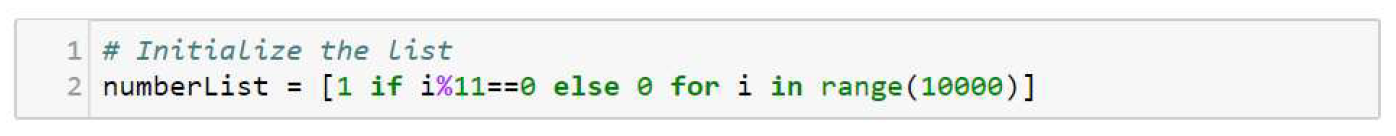
\includegraphics[width=\textwidth]{../IMG/7M05.png} 
\end{figure}
Don’t worry about understanding this line. What you see above is called list comprehension which is not part of the syllabus but used here to quickly generate larger lists for you to work with. The command will produce:
\begin{itemize}
	\item {\code{numberList}} which stores, for every number between 0 and 10,000, whether the
number is divisible by eleven. If the number is divisible 11 eleven, the value in the list
will be one, if the number is not divisible by 11 the number will be 0.
\end{itemize}
Using the {\code{count()}} function, determine how many numbers between 0 and 10,000 are
divisible by 11.\\


\textit{Hints:
Divisibility by 11 corresponds to a list element 1. So you will need to count how many times
the number one is contained in the list.}\\[1cm]


% ------------------------------------------------------------------------------


\subsubsection*{Exercise 7.M06}
Copy the following list into your Jupyter Notebook:
\begin{figure}[H]
		\centering
		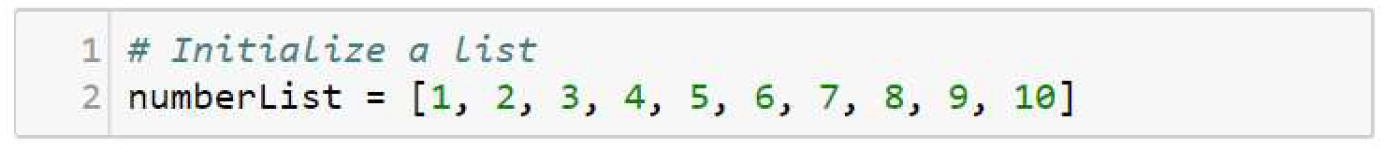
\includegraphics[width=\textwidth]{../IMG/7M06.png} 
\end{figure}
Using the {\code{pop()}} function, write a program that stores the reverse of {\code{numberList}} in a new list {\code{numberListReverse}}.\\


\textit{Hints:
Start with an empty list {\code{numberListReverse}} and fill it using the {\code{pop()}} function on {\code{numberList}} multiple times.}\\[1cm]


% ------------------------------------------------------------------------------


\subsubsection*{Exercise 7.S01}
Start by initializing an empty list. Then ask the user for three cities and append them to the
empty list. Finally check whether London was one of the cities the user entered.\\


\textit{Hints:
You can initialize empty lists by simply leaving out the objects between the square brackets.
You can then either check each list object manually to test whether one of the strings is
"London" or you can use the {\code{in}} function.}\\[1cm]


% ------------------------------------------------------------------------------


\subsubsection*{Exercise 7.S02}
Start with the following list of the London boroughs:
\begin{figure}[H]
		\centering
		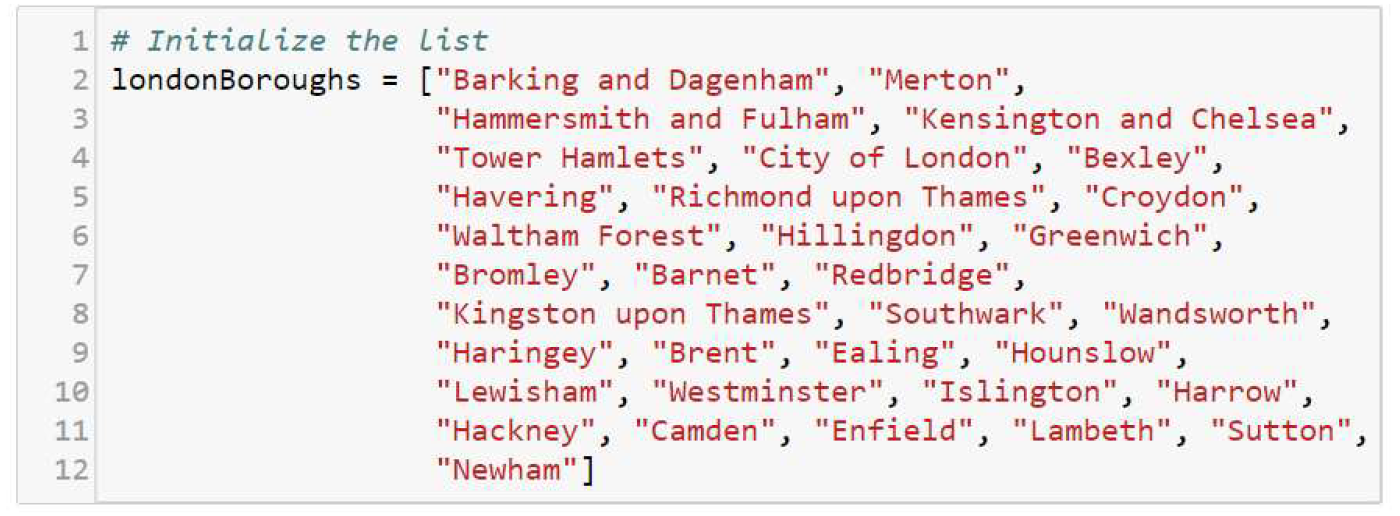
\includegraphics[width=\textwidth]{../IMG/7S02.png} 
\end{figure}
And bring it into alphabetical order.\\


\textit{Hints:
Use Google to figure out whether there is a list operator that can do this for you.}


% ------------------------------------------------------------------------------

\newpage
\section{Difficulty: HARD}

\subsubsection*{Exercise 7.H01}
In your Jupyter Notebook, initialize the following 2-dimensional list:
\begin{figure}[H]
		\centering
		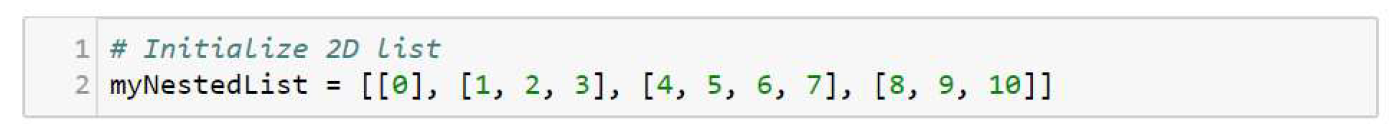
\includegraphics[width=\textwidth]{../IMG/7H01.png} 
\end{figure}
This parent list contains 4 child lists of varying length. Make sure you understand the
structure of this nested list before continuing (sometimes it helps drawing list structures on
a piece of paper).\\
Once you feel like you understand the generated list, continue to the exercises:
\begin{enumerate}[label=(\alph*)]
	\item Using list indices print the first, then the second, then the third, and finally the fourth child list
	\item Using list indices, print out elements 0, 3, 4, and 9
	\item Replace the object 8 with 88
	\item Generate a sub-list containing the elements 4 to 6 and 9 to 10 using list slicing
methods
	\item Append the new child list [11, 12, 13, 14, 15, 16] to the end of the nested
list
	\item Insert the new child list [-2, -1] at index 0 in the nested list
	\item Using the {\code{del}} function, remove the second child list in the nested list
	\item Using the {\code{remove()}} function, remove the elements 4 and 9 from the nested list
	\item Using the {\code{in}} function, check whether the number 10 is in any of the child lists
	\item Using the {\code{len()}} function, determine how many child lists are contained in the parent list
	\item Using the {\code{len()}} function, determine the length of the individual child lists
\end{enumerate}


